\chapter{RFX-Hunch: a closed example based on electron temperature}
\label{section:RFXhunch}
With the aim at selecting an informative example of plasma computation that the machine learning could be devoted to we chose to look at the temperature profiles that are coming from the Soft X-Ray diagnostics at RFX. The particular choice is mainly motivate to provide a example that can be at the same time good representative factor of the plasma global configuration even being at the same time not too complex to be handled by simple networks. The electron temperature profile is a very important clue for the plasma state that is very often accessed by physicists during analysis: it can be seen as an instant property that is almost ergodic during the pulse, it is acquired with a good temporal resolution and can be "easily" related to the magnetic configuration for the chosen sample.

A plasma is composed with a mixture of species characterized by their own mass and electric charge. As first approximation, the plasma may be considered as consisting of two fluids mixed together: the first composed by the electrons and the second by the ions, or to be more specific by all the other heavy species, i.e. ions, neutral atoms, and compound molecules.

What matters for a fusion machine is actually the ions temperature because electrons are not directly involved on fusion process.
Nevertheless electrons acquire energy from the electric field, which energizes the plasma, and lose part of it through elastic or inelastic collisions; in this way the plasma can move energy from one fluid to the other. 
 


\section{What involved ( based on “SCHEMA” )} % SHAx

%% FD-NT-27
\section{Passing from simulated data to actual data  “missing points”  }


\section{( show using of dropout, rebalancing and beta )}


\section{Adding information through models ( Zanca-Terranova )}


\section{parameters to SXR mapping}


\subsection{STEP 12.7}


\begin{figure}
    \centering
    \subfigure{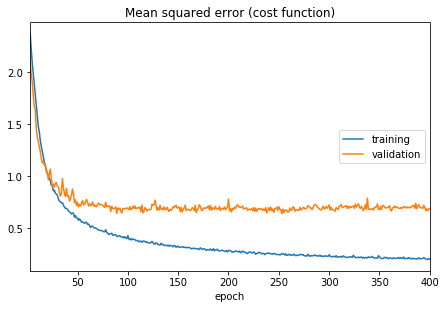
\includegraphics[height=3.3cm]{img/STEP12_7/STEP12_7_pBr2SXR_rm-rs_absarg_training_mse.png} \label{step_12_7_training}}
    \subfigure{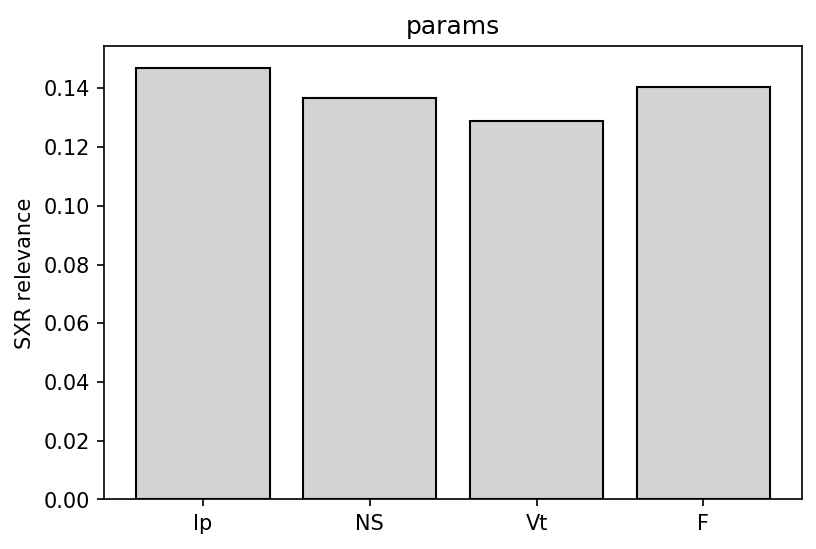
\includegraphics[height=3.3cm]{img/STEP12_7/STEP12_7_params.png} \label{step_12_7_p}}
    \subfigure{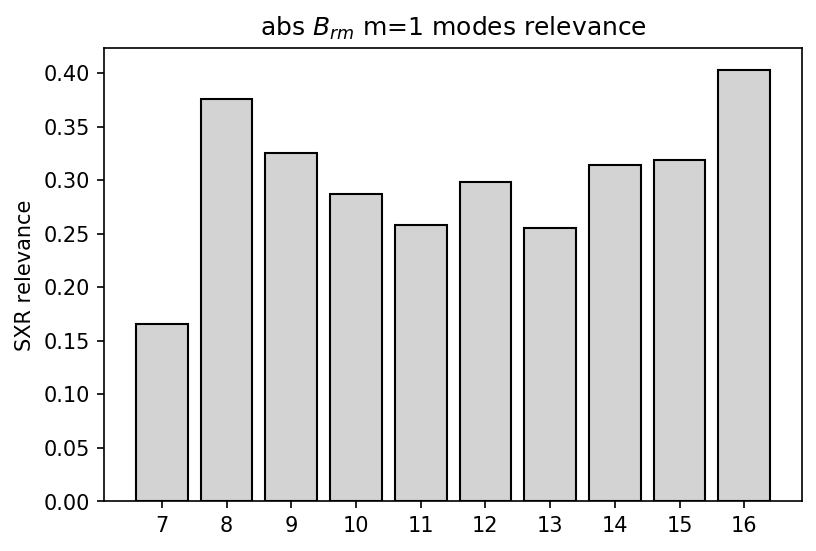
\includegraphics[height=3.3cm]{img/STEP12_7/STEP12_7_abs_Br_rm.png} \label{step_12_7_abs_Brm}}
    \subfigure{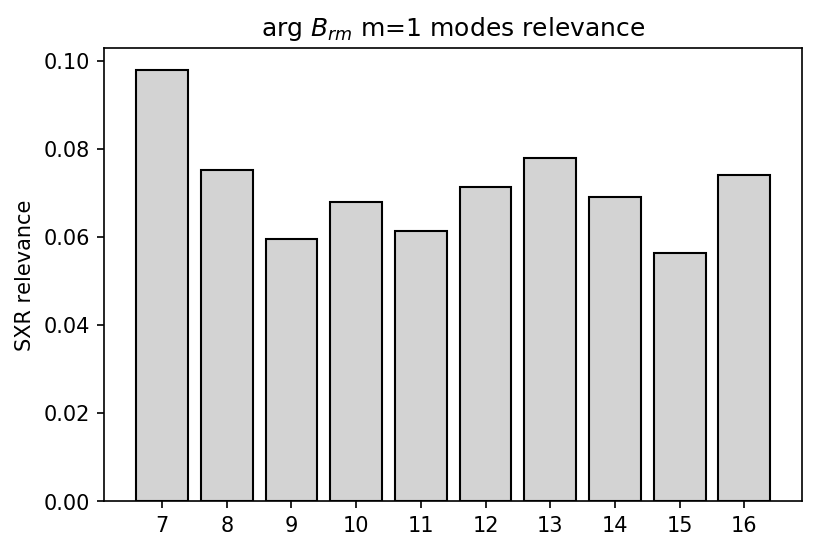
\includegraphics[height=3.3cm]{img/STEP12_7/STEP12_7_arg_Br_rm.png} \label{step_12_7_arg_Brm}}
    \subfigure{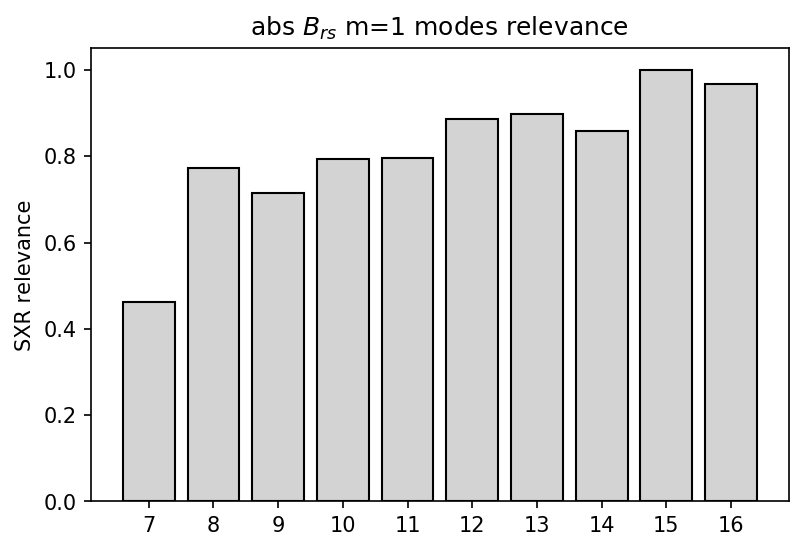
\includegraphics[height=3.3cm]{img/STEP12_7/STEP12_7_abs_Br_rs.png} \label{step_12_7_abs_Brs}}
    \subfigure{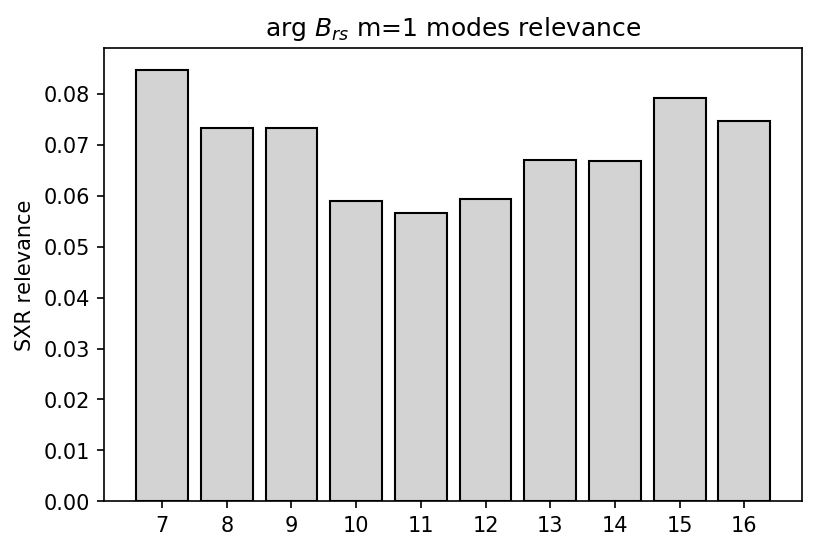
\includegraphics[height=3.3cm]{img/STEP12_7/STEP12_7_arg_Br_rs.png} \label{step_12_7_arg_Brs}}
    \caption{ Training 500 epochs - STEP 12.7 mse, slightly overfitted but validation not diverging }
    \label{fig:step_12_7}
\end{figure}

\begin{figure}
    \centering
    \subfigure{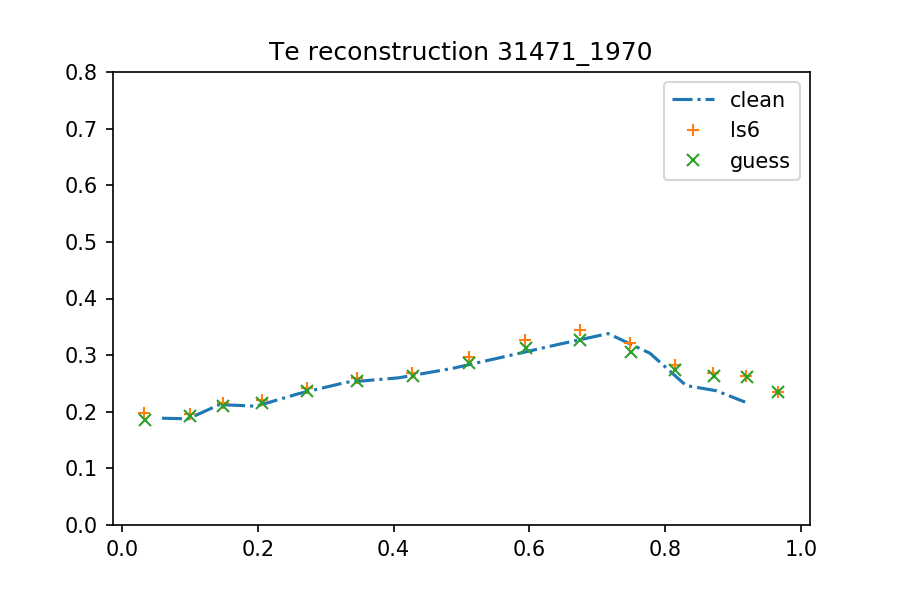
\includegraphics[height=4.8cm]{img/STEP12_7/Te_rec_215.png} }
%   \subfigure{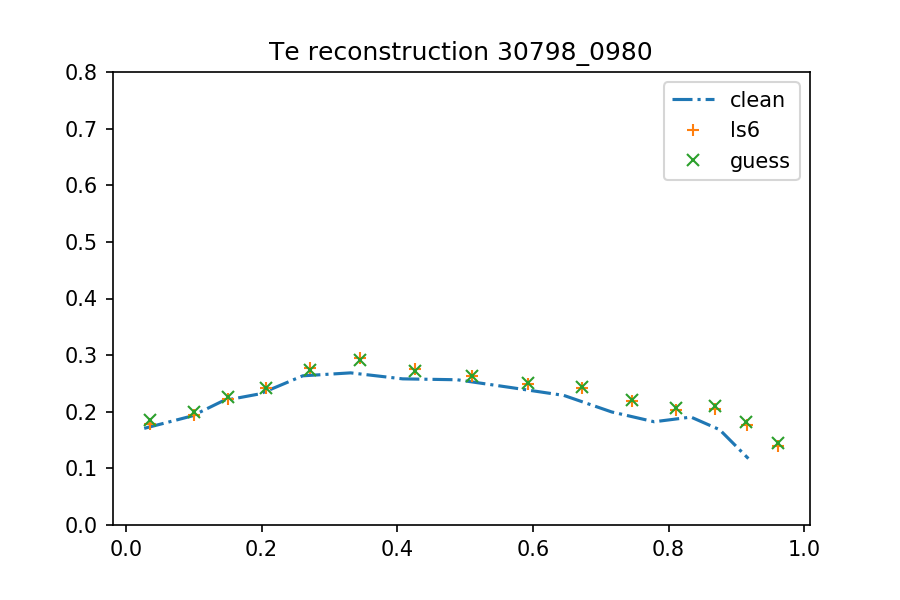
\includegraphics[height=4.8cm]{img/STEP12_7/Te_rec_219.png} }
    \subfigure{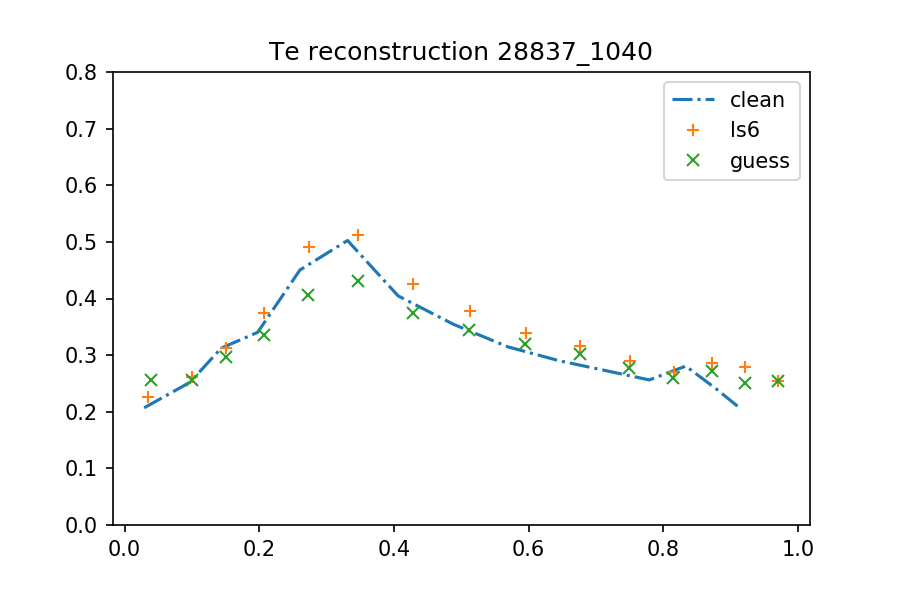
\includegraphics[height=4.8cm]{img/STEP12_7/Te_rec_229.png} }
    \subfigure{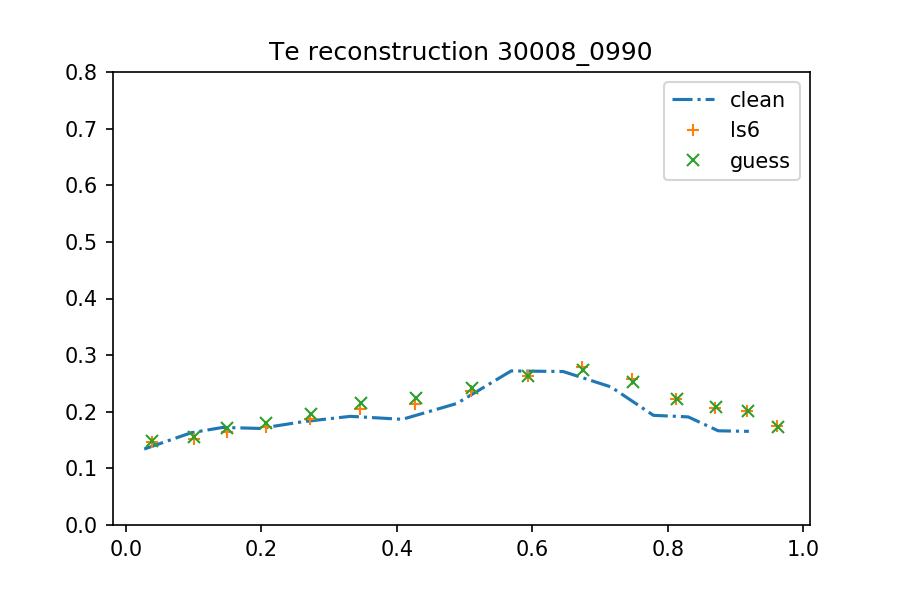
\includegraphics[height=4.8cm]{img/STEP12_7/Te_rec_232.png} }
%   \subfigure{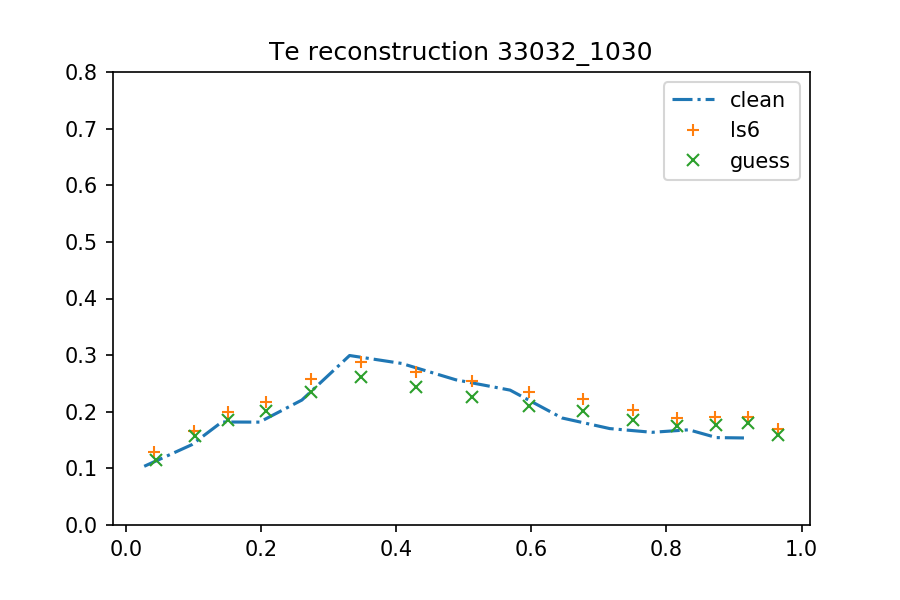
\includegraphics[height=4.8cm]{img/STEP12_7/Te_rec_243.png} }
    \subfigure{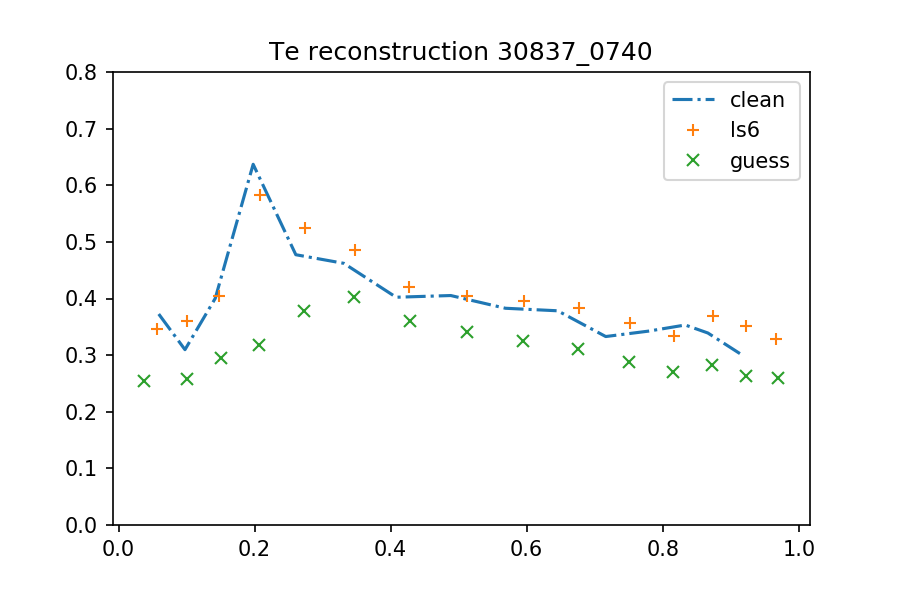
\includegraphics[height=4.8cm]{img/STEP12_7/Te_rec_213.png} }
    \caption{ Training 500 epochs - STEP 12.7 mse, slightly overfitted but validation not diverging }
    \label{fig:step_12_7_rec}
\end{figure}

